\documentclass[aps,pra,twocolumn,10pt]{revtex4-1} % chktex 8
\usepackage{amssymb}
\usepackage{amsfonts}
\usepackage[fleqn,tbtags]{amsmath}
\usepackage{graphicx} 

\newcommand{\function}[1]{f_{\mathrm{#1}}}
\newcommand{\weight}[1]{\lambda_{\mathrm{#1}}}
\newcommand{\BB}{{\{0, 1\}}}

\begin{document}

\title{Quantum Annealing for Air Traffic Management}
\author{Tobias Stollenwerk}
\affiliation{German Aerospace Center, Linder H\"ohe, 51147 Cologne, Germany}
\author{Bryan O'Gorman},
\author{Salvatore Mandr\`{a}}
\author{Eleanor G. Rieffel}
%\author{Davide Venturelli},
%\author{Olga Rodionova},
%\author{Hok K. Ng},
%\author{Banavar Sridhar},
\affiliation{NASA Ames, Moffet Blvd, Mountain View, CA 94035, USA}
\date{\today}


% TODO: remove frontmatter

\thispagestyle{empty}
\tableofcontents
\listoffigures
\clearpage

\maketitle

\section{Introduction}
There is an overall increase in air traffic over the last decades and this trend is believed to continue.
As a result, the air traffic control system is increasingly under pressure.
The current system works with pre-planned routes for the flights and more or less manual conflict avoidance with the help of air traffic controllers.
With the limited airspace available, novel approaches are necessary to meet the demand of even more air traffic in the coming decades.
A promising approach to solve this problem is using wind-optimal trajectories beyond the predefined air traffic network \cite{ng_optimizing_2014}.
However, the conflicts in the wind-optimal trajectories need to be avoided, or ``deconflicted``  \cite{rodionova16}.

Quantum annealing is a promising computational method which became increasingly important in recent years.
This development is driven also by first commercially available quantum annealing device by the company D-Wave Systems.
In addition to studying the fundamental properties of quantum annealing, it is imperative to find possible real world application for this technology.
Hard operational planning problems are a promising candidate for the latter \cite{Rieffel2015, Venturelli2015}.

In this work, we investigate the feasibility of applying quantum annealing to the deconfliction of wind-optimal trajectories. 
In the course of this, we use wind-optimal trajectory data to extract realistic problem instances.
To be amenable to a D-Wave Quantum annealer, the problem has to be formulated as a quadratic unconstrained binary optimization (QUBO) problem.
We demonstrate the mapping of deconfliction problem to a QUBO formulation.
Since restrictions to the configurations space are necessary for the reformulation of the problem as a QUBO, we investigate the influence of this restriction on the solution quality.
Moreover, we study the embeddability and solution quality using both classical solvers and quantum annealing runs.


\section{Problem specification}
\label{sec:problem_specification}

The basic input of the deconflicting problem is a set of ideal flight trajectories (space-time paths).
These ideal trajectories are specified by the individual flight operators.
Each ideal trajectory represents some independent optimization from the operator's perspective, especially minimizing fuel costs given expected wind conditions between the desired origin and destination at the desired times;
for this reason, they are called the ``wind-optimal'' trajectories.
Because of the number of such trajectories and the correlation between them, these trajectories are likely to conflict; that is, two or more aircraft are likely to get dangerously close to each other if their ideal trajectories are followed without modification.
The goal thus is to modify the trajectories to avoid such conflicts.

In theory, the configuration space consists of all physically realistic trajectories; in practice, computational bounds constrain us to consider certain perturbations of the ideal trajectories.
The simplest such perturbation is a departure delay, which is the main focus of the present work.
Previous work~\cite{rodionova16} additionally considered a global perturbation by which a trajectory is sinusoidally shifted parallel to the Earth's surface.
We focus instead on local perturbations to the trajectories, in which a modification to the trajectory is parameterized by some choice of active maneuvers near a potential conflict; such a modification does not affect the preceding part of the trajectory and only affects the subsequent part by the additional delay it introduces.

A full accounting of the cost of such modifications would take into account the cost of departure delays, the change in fuel cost due to perturbing the trajectories, the relative importance of each flight, and many other factors.
As in previous work, we consider only the total, unweighted arrival delay, aggregated equally over all of the flights.

Formally, each ideal trajectory $\mathbf x_i = {\left(x_{i, t}\right)}_{t=t_{i,0}}^{t_{i,1}}$ is specified as a time-discretized path from the departure point $x_{i, t_{i, 0}}$ at time $t_{i, 0}$ to the arrival point $x_{i, t_{i, 1}}$ at time $t_{i, 1}$.
For each flight $i$, the geographical coordinates $x_{i,t}$ (as latitude, longitude, and altitude) are specified at every unit of time (i.e.\ one minute) between $t_{i,0}$ and $t_{i,1}$;
we call this interval $T_i = \left(t_{i,0}, t_{i, 0} + 1, \ldots, t_{i,1}\right)$.

For notational simplicity, suppose momentarily that each trajectory $\mathbf x_i$ is modified only by introducing delays between time steps.
Let $\delta_{i, t}$ be the accumulated delay of flight $i$ at the time that it reaches the point $x_{i, t}$, and let $\delta^*_{i, t}$ be the maximum such delay.

A pair of flights $(i, j)$ are in conflict with each other if any pair of points from their respective trajectories is in conflict.
(The trajectories are reasonably assumed to be sufficiently time-resolved so that if the continuously interpolated trajectories conflict than there is a pair of discrete trajectory points that conflict.)
A pair of trajectory points $(x_{i,s}, x_{j,t})$ conflict if their spatial and temporal separations are both within the respective mandatory separation standards $\Delta_x$ and $\Delta_t$ (i.e.\ $3$ nautical miles and $3$ minutes):
\begin{equation}
\left\|x_{i, s} - x_{j,t}\right\| < \Delta_x \text{ and } 
\left|\left(s + \delta_{i, s}\right) - \left(t + \delta_{j,t}\right)\right|
< \Delta_t
\end{equation}.
The latter condition can be met for some 
$\left(\delta_{i,s}, \delta_{j,t} \right) \in [0, \delta^*_{i,s}] \times [0, \delta^*_{j,t}]$ if and only if 
\begin{equation}
\max \left\{\delta^*_{i, s}, \delta^*_{j, t}\right\} + \Delta_t > |s - t|,
\end{equation}
in which case we call the pair of trajectory points \emph{potentially} conflicting.
The set $C$ of such pairs of potentially conflicting trajectory points contains strongly correlated clusters.
To simplify the constraints, we enumerate all such clusters and refer to them simply as \emph{the} conflicts.
That is, we partition the potentially conflicting pairs of trajectory points into disjoint sets,
\begin{equation}
C =  \bigcup_{k} C_k,
\end{equation}
such that if $\left\{(i, s), (j, t)\right\}, \left\{(i', s'), (j', t')\right\} \in C_k$ for some $k$ then
$i = i' < j = j'$ and for all 
$s'' \in [\min \{s, s'\}, \max\{s, s'\}]$
there exists some 
${t'' \in [\min \{t, t'\}, \max\{t, t'\}]}$
such that
${\left\{(i, s''), (j, t'')\right\} \in C_k}$ and vice versa.
Thus every conflict $k$ is associated with a pair of flights $I_k = \{i, j\}$.
Let $K_i = \left\{k \middle| i \in I_k \right\}$ be the set of conflicts to which flight $i$ is associated, $\Nc$ the number of conflicts, and $\Nf$ the number of flights.

Having identified disjoint sets of conflicts, we relax the supposition that the trajectory modifications only introduce delays between time steps.
Instead, we consider modifications to the trajectories that introduce delays local to particular conflicts.
Specifically, the configuration space consists of the departure delays $\mathbf d = {\left(d_i\right)}_{i=1}^{\Nf}$ and the set of local maneuvers $\mathbf a_{\mathbf k} = {\left(\mathbf a_k\right)}_k$, where $\mathbf a_k$ represents some parameterization of the local maneuvers used to avoid conflict $k$.
Let $d_{i, k} (\mathbf d, \mathbf a_{\mathbf k})$ be the delay introduced to flight $i$ at conflict $k$, as a function of the departure delays and local maneuvers.
With this notation, we can write the total delay as
\begin{equation}
D = 
\sum_{i = 1}^{\Nf}
\left(d_i + \sum_{k \in K_i} d_{i, k}\right).
\end{equation}
This is the quantity we wish to minimize subject to avoiding all potential conflicts.
\begin{figure}[htpb]
    \begin{center}
        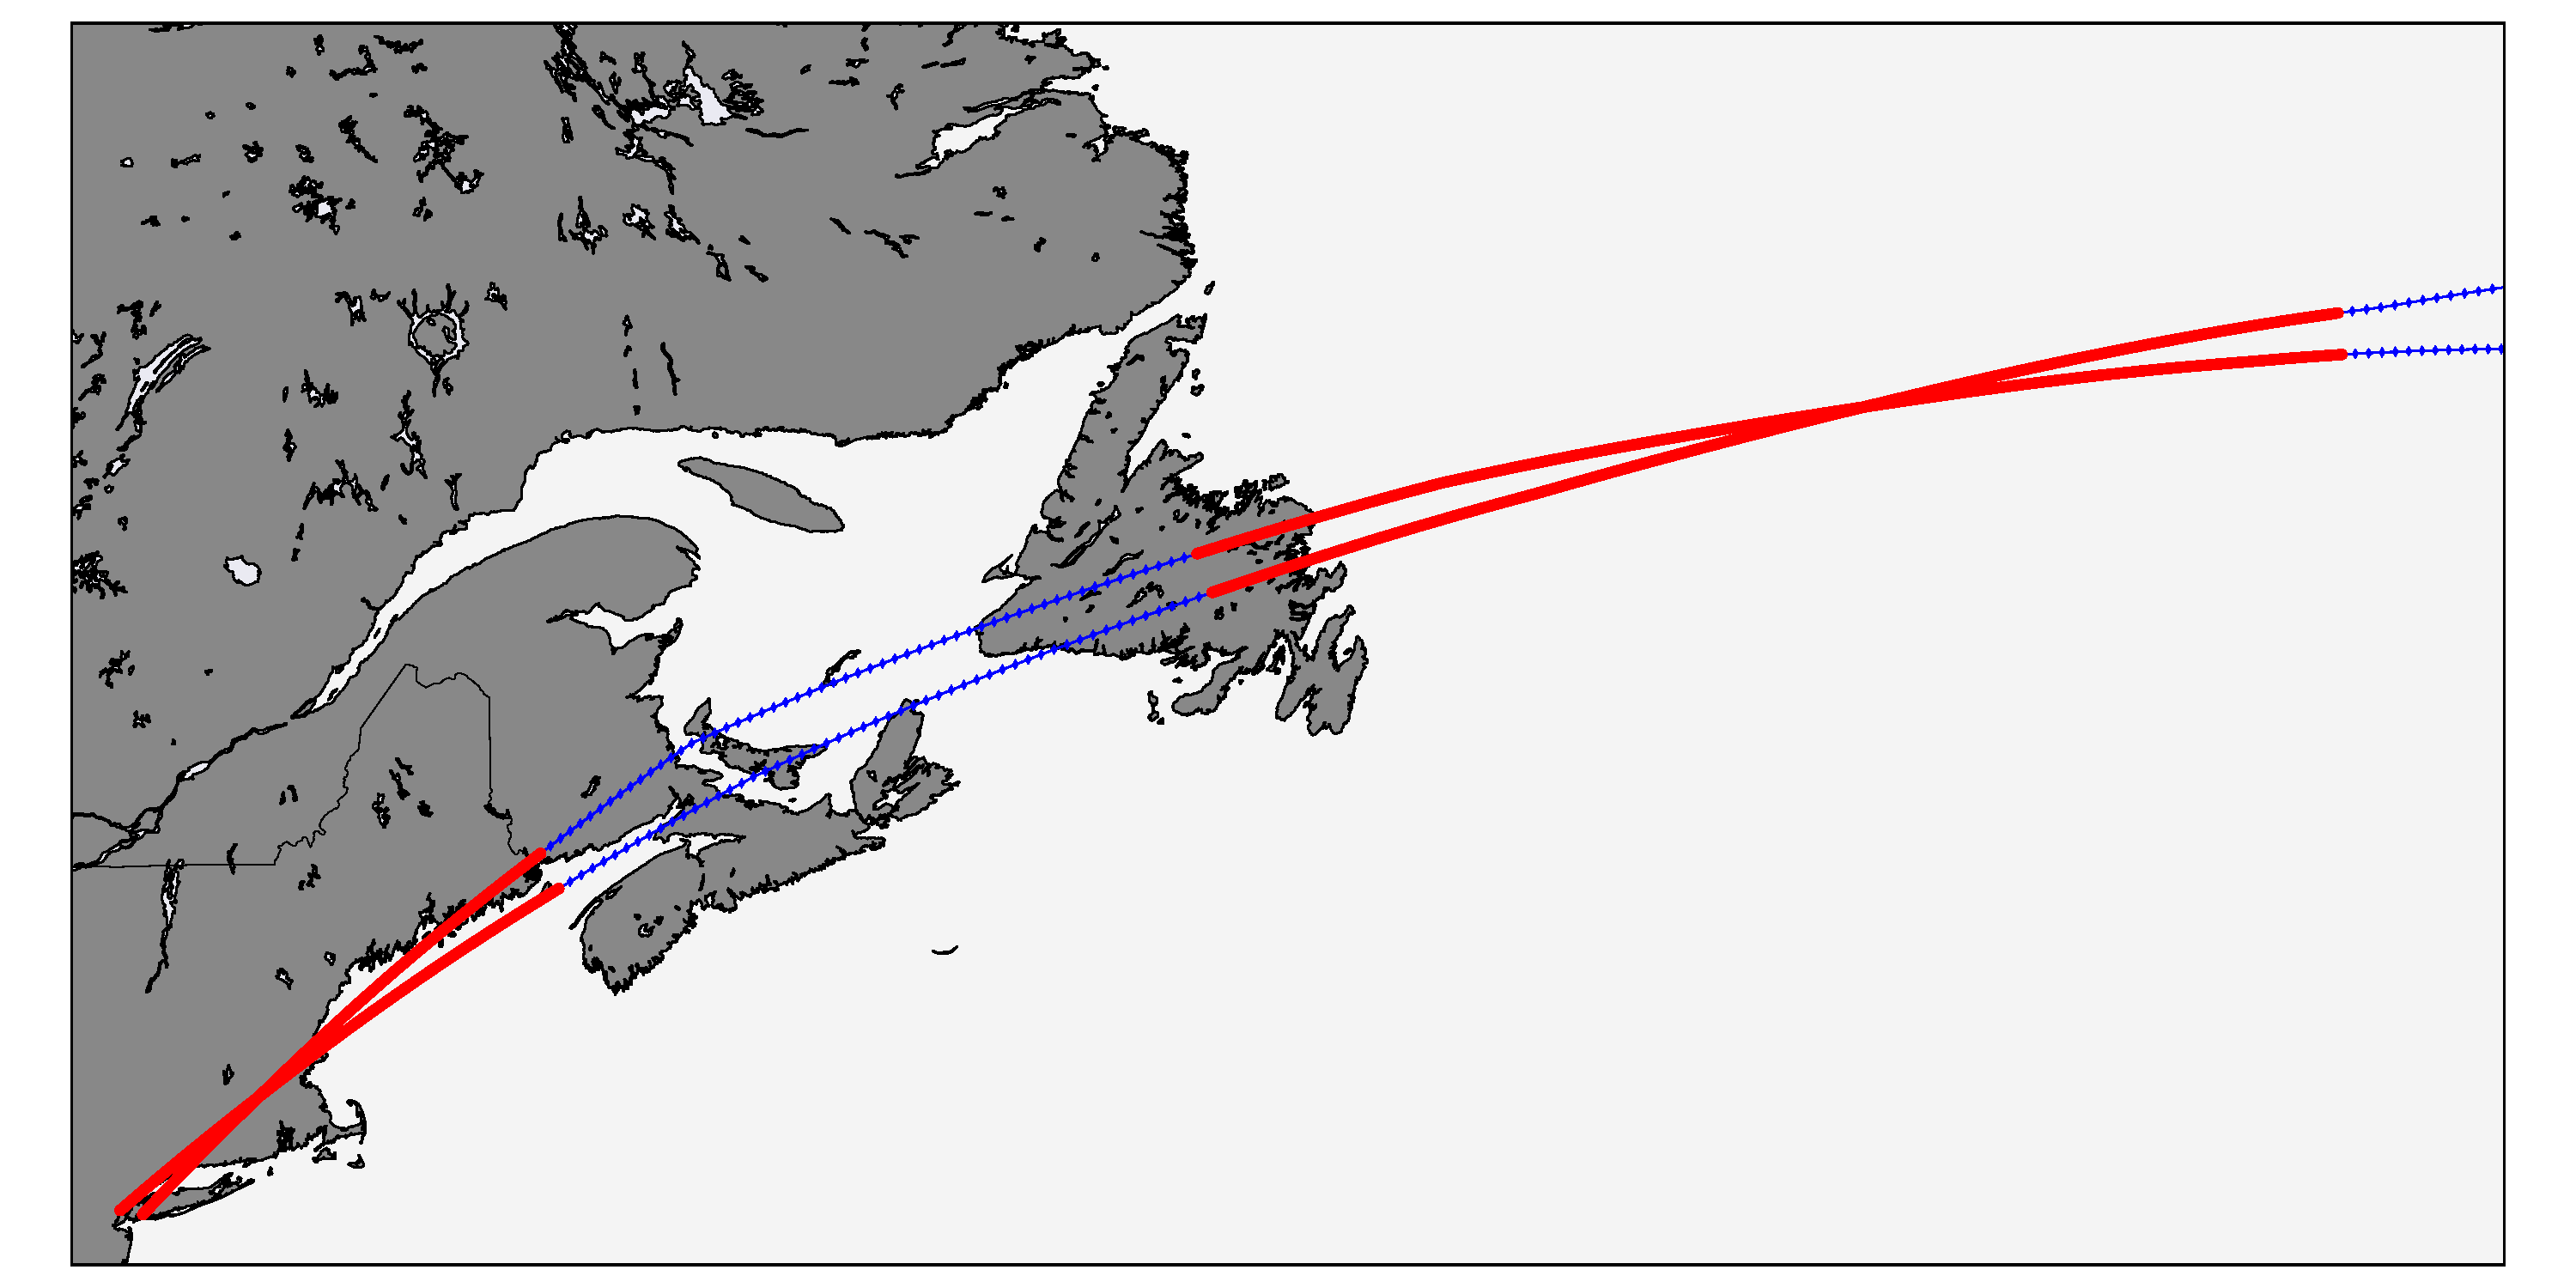
\includegraphics[width=0.45\textwidth]{./pics/example_conflict_in_real_space.pdf}
    \end{center}
    \caption[Conflict example]{Example of two parallel potential conflicts between two transatlantic flights starting from the east cost of the USA.}
\label{fig:example_parallel_conflict}
\end{figure}

%\begin{figure}[htpb]
%    \begin{center}
%        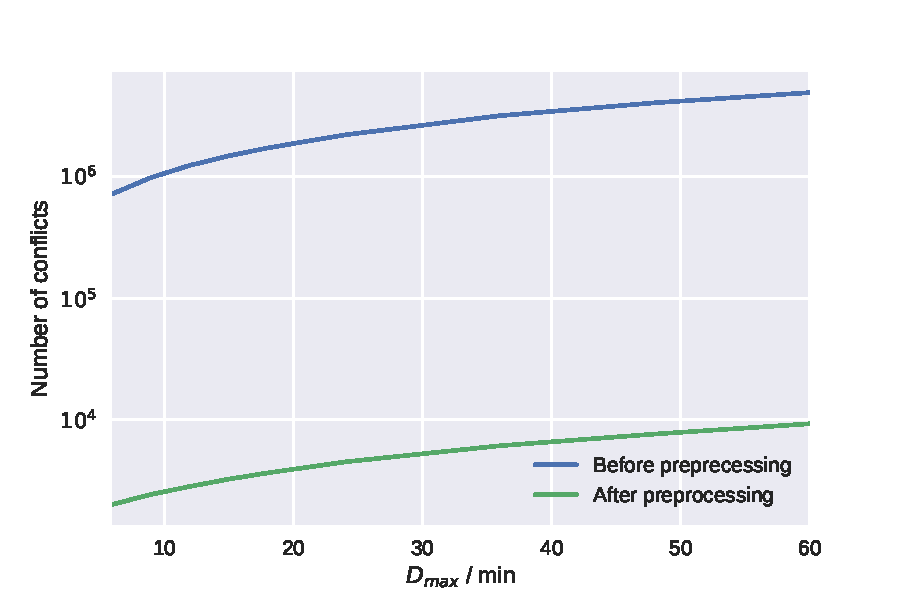
\includegraphics[width=0.45\textwidth]{./pics/preprocessing_reduction_number_of_conflicts.pdf}
%    \end{center}
%    \caption[Conflict preproccesing]{Preprocessing: Reduction in the number of potential conflicts for various upper delay bounds $D_\text{max}$.}
%\label{fig:preprocessing_reduction_number_of_conflicts}
%\end{figure}

A conflict can be avoided locally by introducing earlier delays differentially, thereby increasing the temporal separation; by some active maneuver of one or both of the flights; or by some combination thereof.
We focus on the former case.
Let 
\begin{equation}
\label{eq:accum-delay}
D_{i, k} = d_i + \sum_{k' \in K_{i, k}} d_{i,k'}
\end{equation}
be the accumulated delay of flight $i$ by the time it reaches conflict $k$,
where $K_{i, k} = \left\{k' \in K_i \middle| k' < k\right\}$.
In this case, $\delta_{i, s} = D_{i, k}$ for all $s$ associated with flight $i$ in conflict $k$.
We assume that the set of conflicts $K_i$ associated with flight $i$ is indexed in temporal order, i.e.\ if $k' < k$ and $k, k' \in K_i$, then flight $i$ reaches conflict $k'$ before conflict $k$.
The pairs of conflicting trajectory points associated with conflict $k$ are given by 
\begin{equation}
T_k = 
\left\{
(s, t) \middle| \{(i, s), (j, t)\} \in C_k, i < j
\right\}.
\end{equation}
Thus the potential conflict is avoided only if 
\begin{equation}
\label{eq:accum-delay-diff}
D_k = D_{i, k} - D_{j, k}
\notin
B_k 
\end{equation}
where 
\begin{align}
B_k &= 
\bigcup_{(s, t) \in T_k}
\left(-\Delta_t + t - s, \Delta_t + t - s\right)
=
[\Delta^{\min}_k, \Delta^{\max}_k], \\
\Delta^{\min}_k &= 1 - \Delta_t + \min_{(s, t) \in T_k} \{t - s\},\\
\Delta^{\max}_k &= \Delta_t - 1 + \max_{(s, t) \in T_k} \{t - s\}.
\end{align}

%In the absence of active maneuvers to avoid conflicts, the deconflicting problem can be summarized as minimizing the total delay $D$ subject to

In the remainder of this paper, we focus on the restricted problem in which only departure delays are allowed.
In this simplified case, the configuration space is simply 
$\mathbf d = {\left(d_i\right)}_{i=1}^{\Nf}$, the cost function simply $D = \sum_{i = 1}^{\Nf} d_i$, and the constraints simply $d_i - d_j \notin B_k$ for all $k$.

\section{Instances}\label{sec:instances}
To assess our methods on realistic instances of the problem, we use the actual wind-optimal trajectories for transatlantic flights on July 29, 2012, as was done in previous work~\cite{rodionova16}.
In these trajectories, each flight has a constant (cruising) altitude 
and constant speed, to within (classical) machine precision,
though our methods generalize to instances without these special properties.

One perspective into the nature of an instance of the deconflicting problem is the \emph{conflict graph}, whose vertices correspond to flights and which has an edge between a pair of vertices if there is at least one potential conflict between the corresponding flights.
Note that the conflict graph for a given set of trajectories depends on the parameters of the problem.
In the case of only departure delays, whether or not a potential conflict, and thus an edge in the conflict graph, exists between two flights is a function of $d_{\max}$.
For a certain value of $d_{\max}$, the conflict graph may contain several connected components, which can be considered as smaller, independent instances.
Figure~\ref{fig:num-CCs-vs-dmax} shows this dependence of the number of connected components on the maximum delay $d_{\max}$,
and Figure~\ref{fig:hist-CC-sizes} shows the distribution of the sizes of the connected components for various values of $d_{\max}$.
Interestingly, 
most of the connected components are very small; for example, with $d_{\max}= 60$ minutes, approximately $75\%$ of the connected components contain no more than $10$ flights.

\begin{figure*}[p]
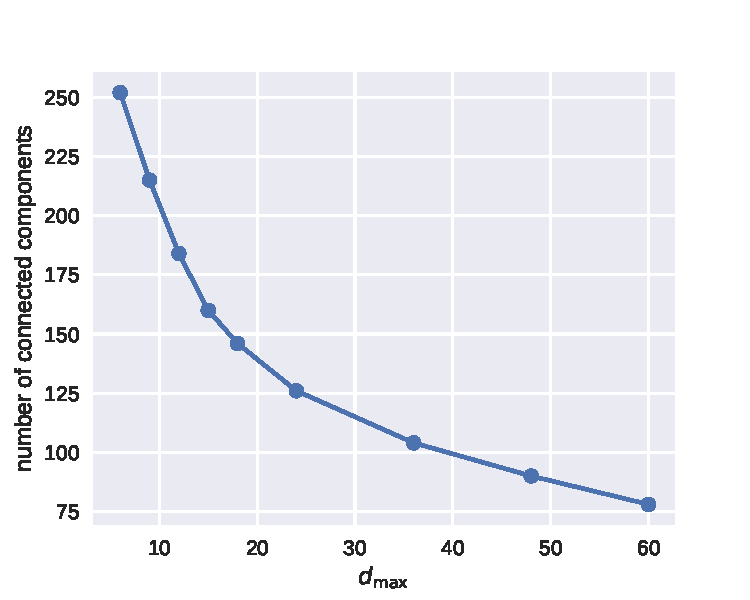
\includegraphics[width=\columnwidth]{pics/instances/num_cc.pdf}
\caption[Number of connected components vs. $d_{\max}$]{Number of connected components versus $d_{\max}$.}
\label{fig:num-CCs-vs-dmax}
\end{figure*}

\begin{figure*}[p]
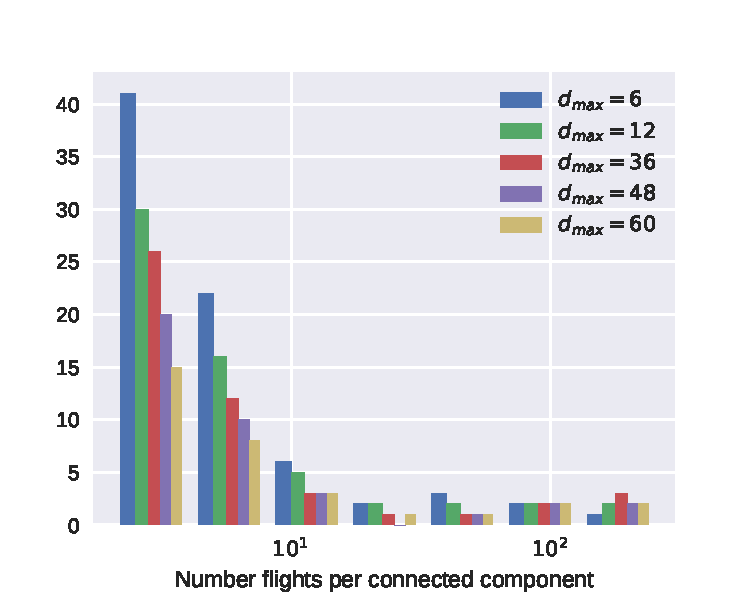
\includegraphics[width=\columnwidth]{pics/instances/analysis_cc.pdf}
\caption[Histogram of connected component sizes]{Histogram of the number of flights per connected component, regardless the maximum delay time.}
\label{fig:hist-CC-sizes}
\end{figure*}

As part of our analysis, we also studied the probability
distribution of the connectivity, namely the number of flights
for which a given flight share a potential conflict with. 
Figure~(\ref{fig:hist-degree}) shows
the distribution of degrees in the conflict graph for $d_{\max}=60$,
which seem to be approximately distributed according to a power law, i.e. 
the number of vertices with degree $d$ is proportional to $d^{\alpha}$.
This is consistent with a so-called ``small-world'' model believed to be typical of many real-world graphs~\cite{barabasi:99}, which are generated by preferential attachment and resultingly contain a few number of highly-connected hubs, as is the case with air traffic.
Figure~(\ref{fig:exponent-vs-dmax}) shows the dependence of this empiral power-law exponent $\alpha$ as a function of $d_{\max}$.
As $d_{\max}$ increases, the exponent decreases.
The larger the delay, the less the structure of the trajectories matters and the flatter the distribution of degrees in the conflict graph.

\begin{figure*}[p]
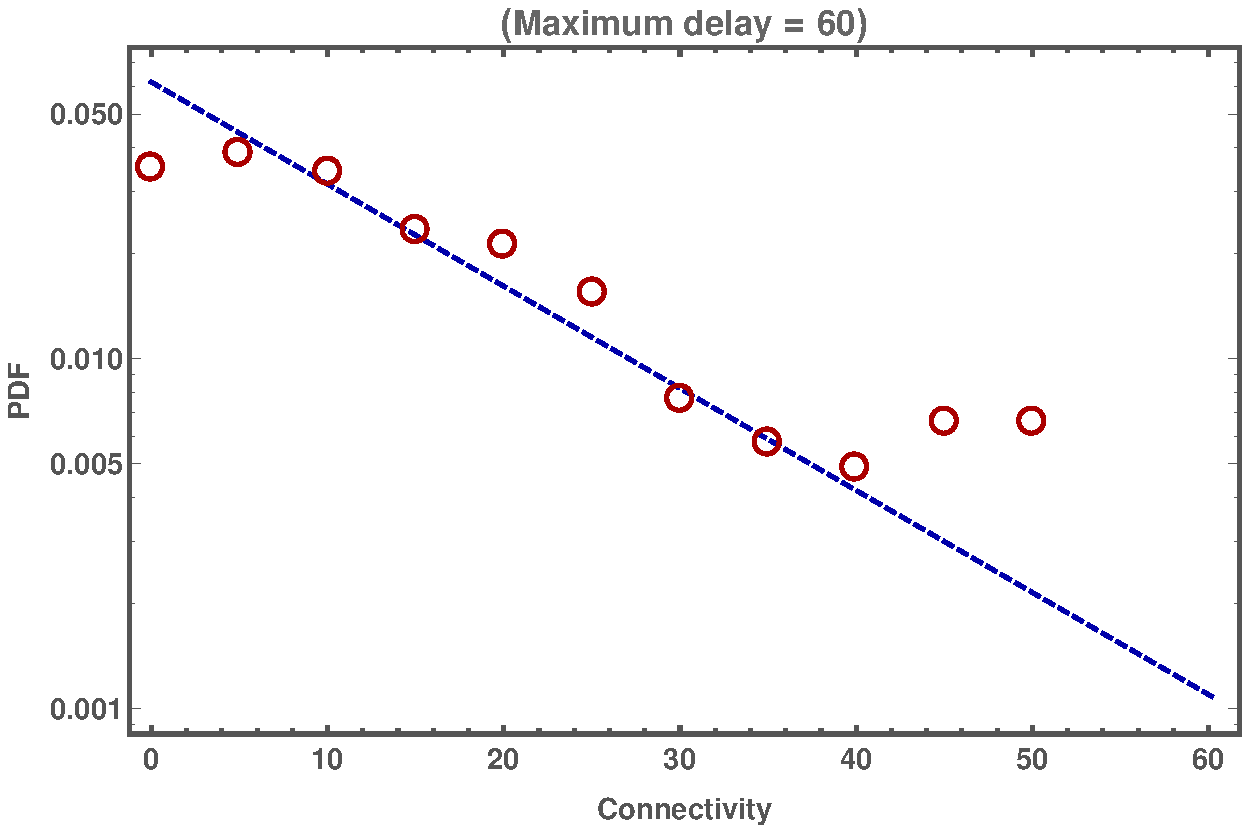
\includegraphics[width=0.95\columnwidth]{pics/instances/connectivity_pdf.pdf}
\caption[Histogram of degrees]{Histogram of the degrees of vertices in the conflict graph for $d_{\max} = 60$. 
The distribution of the degrees approximately follows a power law, with the exponent depending on $d_{\max}$.
}
\label{fig:hist-degree}
\end{figure*}

\begin{figure*}
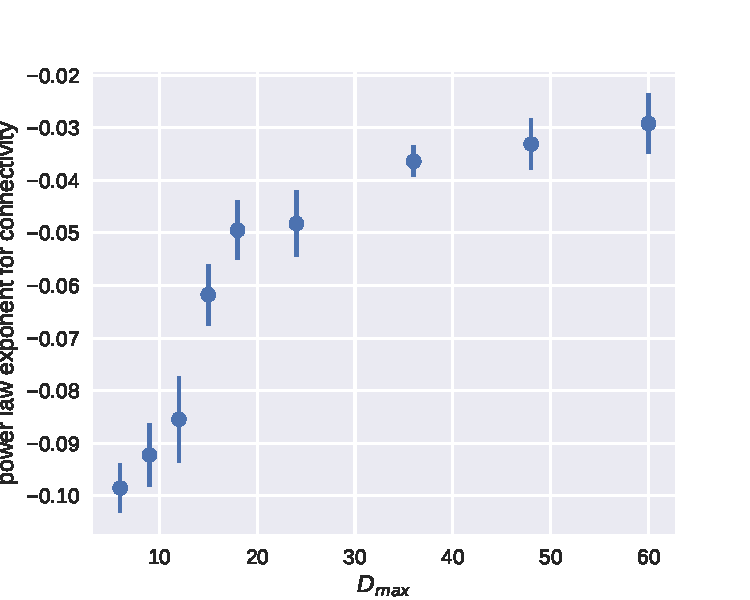
\includegraphics[width=0.95\columnwidth]{pics/instances/connectivity_pl.pdf}
\caption[Power-law exponent vs. $d_{\max}$]{Empirical power-law exponent versus $d_{\max}$.}
\label{fig:exponent-vs-dmax}
\end{figure*}

In many cases, generally hard problems are easy when restricted to tree-like instances~\cite{bertele1972, halin1976s}.
For example, if the conflict graph here is a tree, then the optimum could be easily found by propogating the delays along the tree;
on the other hand, if the conflict graph is a complete graph, finding the optimum is much harder.
The tree-width of a graph formalizes this notion of tree-likeness, ranging from $1$ for a tree to $n-1$ for fully connected graph.
We examine the treewidth of the connected components as a proxy for the hardness of the instances they represent.
Figure~\ref{fig:hist-tws} shows that most connected components are very tree-like, while there are a few strongly-connected components.

\begin{figure}
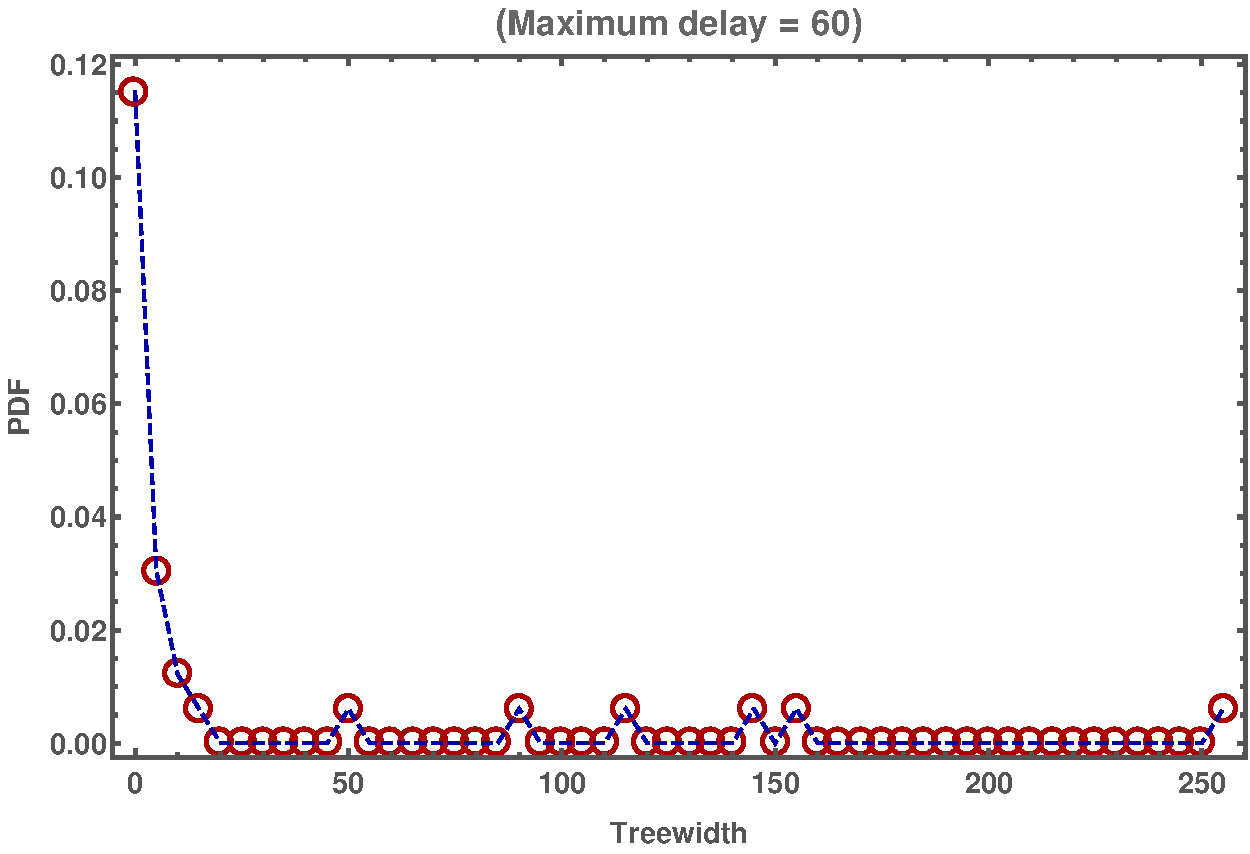
\includegraphics[width=\columnwidth]{pics/instances/treewidth_histogram.pdf}
\caption[Histogram of connected component treewidths]{Histogram of the treewidths of the connected components of the conflict graph for various values of $d_{\max}$.}
\label{fig:hist-tws}
\end{figure}

Figure~\ref{fig:tw-vs-CC-size} shows that the treewidth of a connected component scales approximately linearly with its size.
This indicates that realistic instances of the deconflicting are indeed hard, and not restricted to easier (bounded tree-width) instances of the generally hard problem.
Moreover, the correlation $\gamma$ between the tree-width of a connected component and its size increases with $d_{\max}$, as shown in Figure~\ref{fig:treewidth-size-correlation}.
The larger $d_{\max}$, the more potential conflicts there are;
restricting $d_{\max}$ also restricts the number of conflicts.

\begin{figure*}
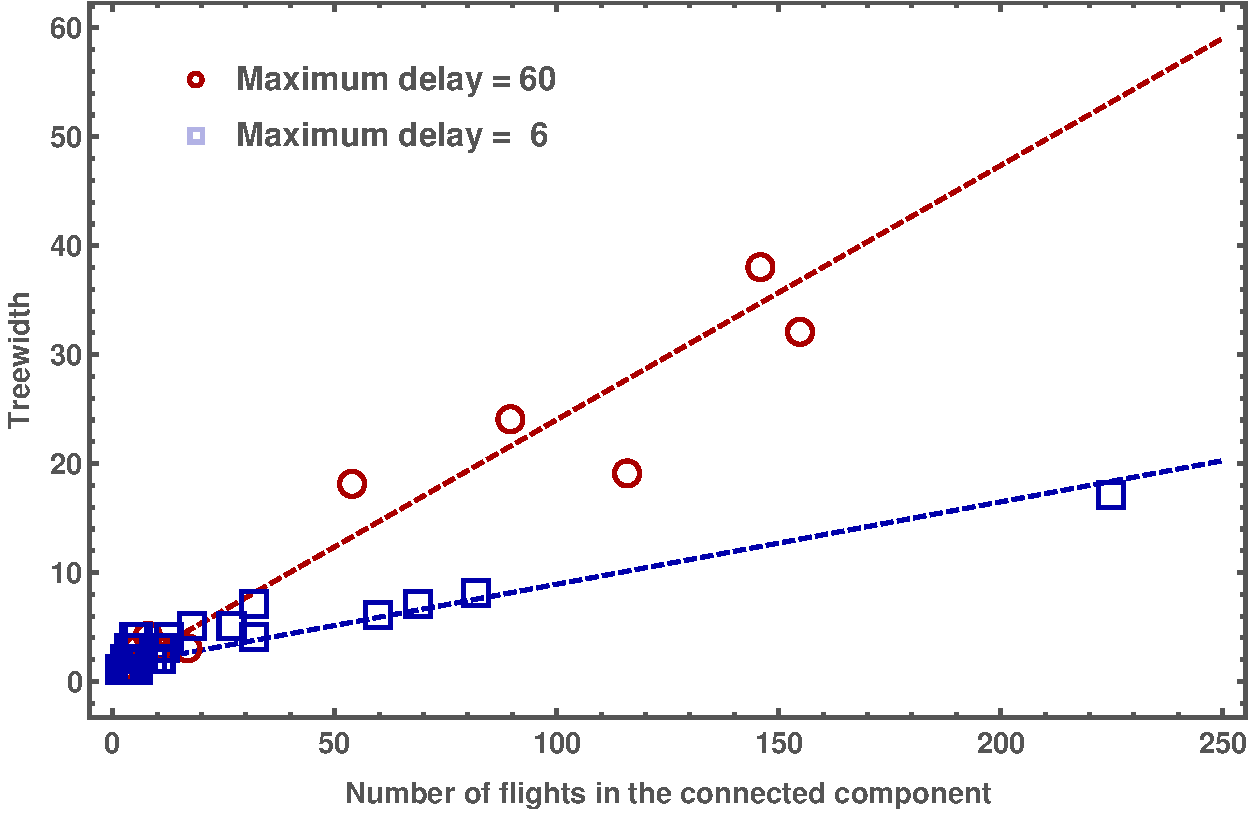
\includegraphics[width=\columnwidth]{pics/instances/treewidth_connectivity.pdf}
\caption[Correlation between connected component size and treewidth]{
The treewidths of connected components versus their sizes for various values of $d_{\max}$.
The correlation is approximately linear, with a slope $\gamma$ that depends on $d_{\max}$.
}
\label{fig:tw-vs-CC-size}
\end{figure*}

\begin{figure*}
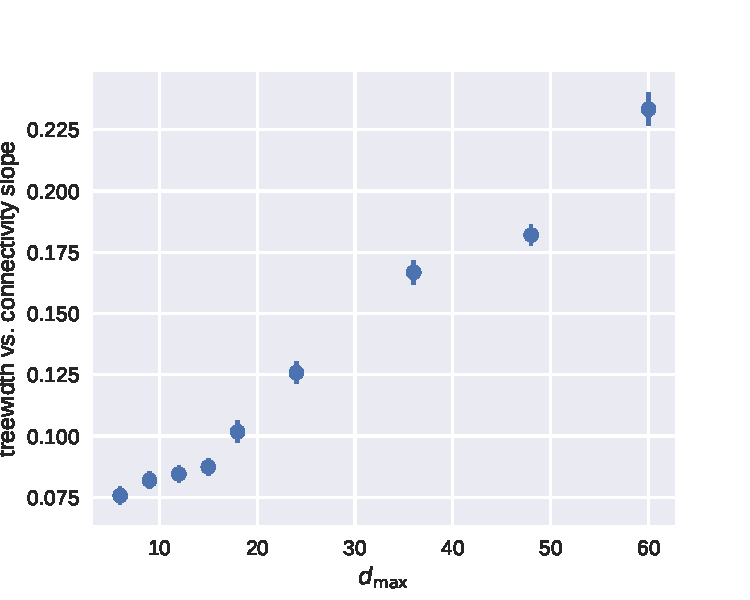
\includegraphics[width=\columnwidth]{pics/instances/treewidth_pl.pdf}
\caption[Treewidth-size correlation coefficient vs. $d_{\max}$]{Slope $\gamma$ as a function
  of the maximum delay time.}
\label{fig:treewidth-size-correlation}
\end{figure*}

\section{Discretizing the configuration space}
It is important to understand how the restrictions to the configuration space by~\eqref{eqn:departure_delay_model_discretization} influence the solution quality.
Therefore we solve~\eqref{eqn:departure_delay_model} with a constraint programming solver~\cite{numberjack} for various delay discretizations and upper bounds as well as for the continuous problem.
As problem instances we used most of the connected components of the conflict graph for $D_\text{max}=18$ minutes with up to $N_f=50$ flights and $N_c=104$ conflicts.
\begin{figure}[htpb]
    \centering
    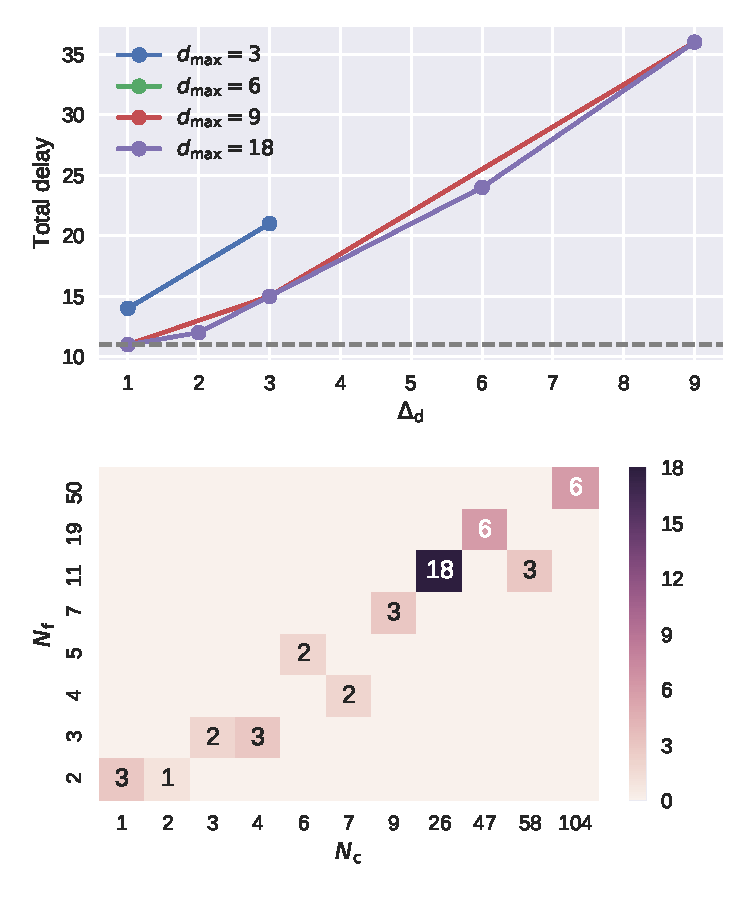
\includegraphics[width=0.45\textwidth]{./pics/delay_only_cp_results.pdf}
    \caption{Top: Total delay of constraint programming solutions for a problem instance with $N_f=19$ flights and $N_c=47$ conflicts for various discretization parameters.
    Bottom: Minimum $d_\text{max}$ which yield optimal solution in continuous problem for various problem instances. For all problem instances we used $D_\text{max}=18$ minutes.}
\label{fig:delay_only_cp_results}
\end{figure}

In Figure~\ref{fig:delay_only_cp_results} one can see the results for a problem instance extracted from a connected component of the conflict graph with $N_f=19$ flights and $N_c=47$ conflicts.
With the exception of the small maximum delay $d_\text{max} = 3$ min, the total delay of the solutions is nearly independent of the maximum delay.
Moreover it is monotonically increasing with the coarseness of the discretization.
Since the original data is discretized in time in units of $1$ minute, $\Delta_t=1$ yield the same result as a continuous variable with the same upper bound.
Obviously the total delay for the continuous solution decreases monotonically with $d_\text{max}$.
Above a certain value $d^0_\text{max}$ the total delay stays the same.
With one exception, we found that for all the investigated problem instances $d^0_\text{max}\leq6$ minutes (see Figure~\ref{fig:delay_only_cp_results}).
Therefore we conclude, that a moderate maximum delay is sufficient even for larger problem instances.
On the other hand, the delay discretization should be as fine as possible to obtain a high quality solutions.

\section{Mapping to QUBO}
\label{sec:mapping}
In this section, we describe how to map to QUBO from the deconflicting problem restricted to only departure delays; a more general mapping is found in the appendix.

\subsection{Binary encoding}
Having suitably discretized the configuration space, we must then encode it into binary-valued variables.
The value of $d_i$ is encoded in $N_d + 1$ variables $d_{i,0}, \ldots, d_{i,N_d + 1} \in \BB$ using a one-hot encoding:
\begin{equation}
d_{i, \alpha} = \begin{cases}
1, & d_i = \alpha,\\
0, & d_i \neq \alpha;
\end{cases}
\qquad
d_i = \Delta_d \sum_{l = 0}^{N_d} d_{i,l}.
\end{equation}
To enforce this encoding, we add the penalty function
\begin{equation}
\label{eq:dep-delay-encoding-penalty}
\function{encoding} = 
\weight{encoding} 
\sum_{i = 1}^n 
{\left(
\sum_{l = 0}^{N_d} d_{i,l} - 1
\right)}^2,
\end{equation}
where $\weight{encoding}$ is a penalty weight sufficiently large to ensure that any cost minimizing state satisfies $\function{encoding} = 0$.
In terms of these binary variables, the cost function is 
\begin{equation}
\label{departure_delay_model_qubo_departure}
\function{delay} = 
\Delta_d
\sum_{i=1}^n 
\sum_{l=0}^{N_d} d_{i,l},
\end{equation}
Lastly, actualized conflicts are penalized by 
\begin{equation}
  \function{conflict}
=
\weight{conflict}
\sum_{k}
\sum_{\substack{\left.l, l' \middle| \Delta_d (l - l') \in D_k\right.\\
\left. i, j \in I_k \middle| i < j \right.}}
  d_{i,l} d_{j, l},
\end{equation}
where again $\weight{conflict}$ is a sufficiently large penalty weight. 
The overall cost function to be minimized is 
\begin{equation}
f
=
\function{encoding} + \function{delay} + \function{conflict}.
\end{equation}


\subsection{Softening the constraints}
The contributions from~\eqref{eqn:departure_delay_model_qubo_unique} and~\eqref{eqn:departure_delay_model_qubo_conflict} to the QUBO for the departure delay model of section~\ref{sec:departure_delay_model} are hard constraints. % chktex 44
This means a solution to the QUBO is only valid if both~\eqref{eqn:departure_delay_model_qubo_unique} and~\eqref{eqn:departure_delay_model_qubo_conflict} vanish.
Therefore, the penalty weights $\lambda_\text{unique}$ and $\lambda_\text{conflict}$ must be chosen sufficiently large to ensure that the hard constraints are fulfilled for the solution to the problem.
On the other hand, large penalty weights lead to large differences between the largest and smallest non-vanishing coefficients in the QUBO.\@
Since the D-Wave quantum annealers have a limited resolution for the specification of the QUBO, this can lead to a misspecification of the problem.
\footnote{Reference to D-Wave limited resolution}
Hence, it is desirable to find a sweet spot of the smallest penalty weights which still yield valid solutions.

\begin{figure}[htpb]
    \centering
    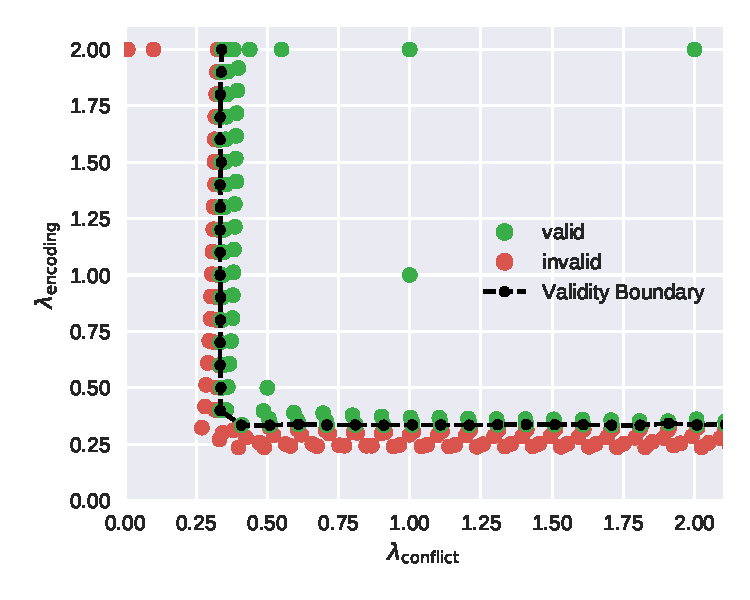
\includegraphics[width=0.45\textwidth]{./pics/validity_boundary_example.pdf}
    \caption{Validity of exact solution to a QUBO extracted from a problem instance with $N_f=7$ flights and $N_c=9$ conflicts in dependence on the choice of the penalty weights, $\lambda_\text{unique}$ and $\lambda_\text{conflict}$. Here, $\Delta_t=3$ and $d_\text{max}=18$.}
\label{fig:penalty_weights}
\end{figure}

In order to find these optimal penalty weights, we employed an exact solver
\footnote{Reference to mapping from QUBO to max sat and to akmaxsat solver} to explore the validity of a solution in dependence on the penalty weights.
We investigated problem instances with up to $N_f=7$ flights and $N_c=9$ conflicts.
For all these problem instances we found a box like shape of the boundary between valid and invalid solutions as it is depicted in figure~\ref{fig:penalty_weights}.

One can give an upper bound for the sufficiently large penalty weights by the following considerations.
A minimal violation of the hard constraints yield an additional contribution to the QUBO cost function of $\lambda_\text{unique}$ or $\lambda_\text{conflict}$, respectively.
Such a violation would correspond to single bit flip in the binary delay variables $d_{i\alpha}$.
Therefore the contribution from~\eqref{eqn:departure_delay_model_qubo_departure} would be reduced maximally by 
\begin{equation*}
    \min_\alpha \frac{-\alpha}{d_\text{max}} = - 1    
\end{equation*}
Hence, sufficiently large penalty weights must fulfill the following conditions
\begin{align*}
    \lambda_\text{unique} & > 1 \\
    \lambda_\text{conflict} &> 1 \, .
\end{align*}
This corresponds to a box like shape as it appears in figure~\ref{fig:penalty_weights}.


\subsection{Solving QUBO instances using ICM}

In this section we present the results for the optimization of the QUBO
formulation of the ATM problem using the Isoenergetic Cluster Method (a
rejection-free cluster algorithm for spin glasses that greatly improves
thermalization)~\cite{zhu2015}, which has been shown to be one of the fastest
classical heuristic to optimize QUBO problems~\cite{mandra2016}.\\

Figure~(\ref{fig:icm1}) shows the total delay time optimized by ICM either by 
varying the partition at fixed the delay step $\Delta t$ (left panel) or by
varying the delay step $\Delta t$ at fixed partition (right panel). As one can
see, the total delay decreases by decreasing $\Delta t$ and it eventually
reaches an optimal plateau. Results are for maximum delay of 60 minutes. This is
consistent with the idea that smaller $\Delta t$ allows a finer optimization of
the delays of the flights.\\

\begin{figure*}
  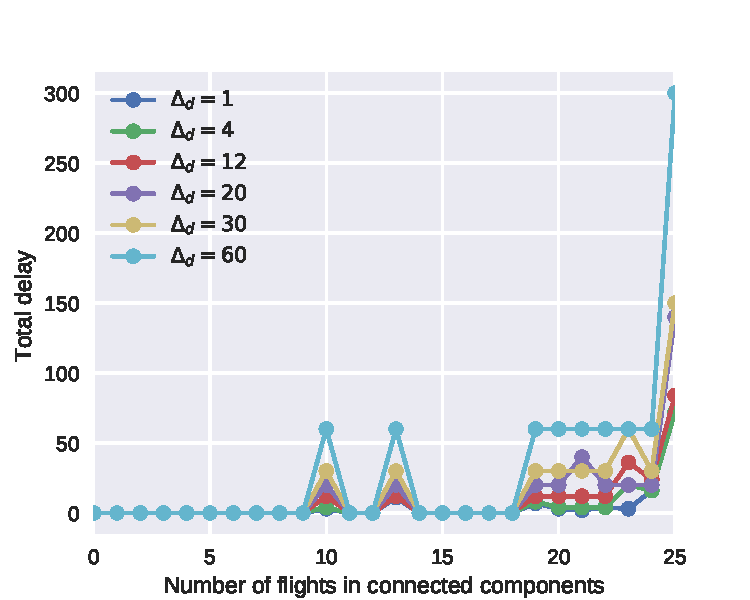
\includegraphics[width=\columnwidth]{pics/qubo_icm/qubo_icm_3.pdf}
  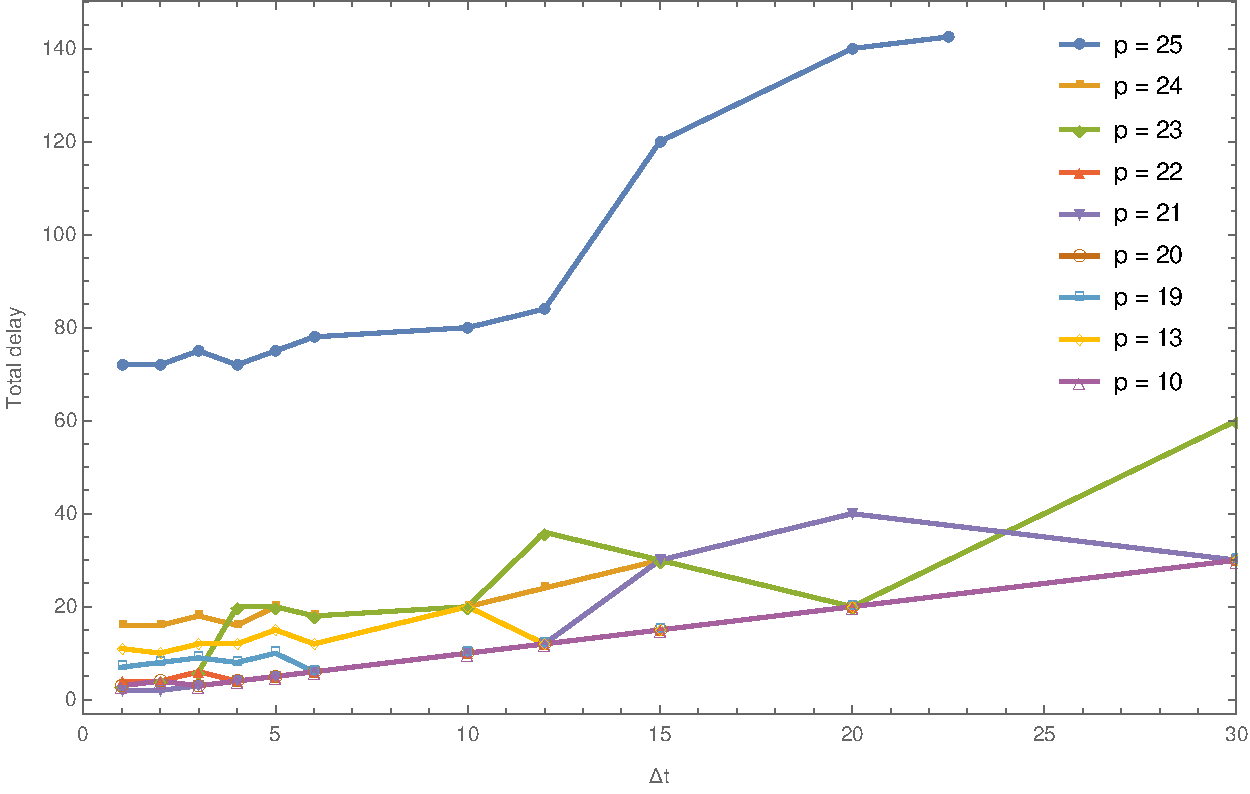
\includegraphics[width=\columnwidth]{pics/qubo_icm/qubo_icm_4.pdf}
  \caption{(Left) Optimal total delay found by using the
  Isoenergetic Cluster Method (ICM) at fixed time step $\Delta t$, by varying
  the connected component. Results are for maximum delay time of $60$ minutes. (Right)
  Optimal delay found by using ICM at fixed connected component, by varying the time step
  $\Delta t$.}
\label{fig:icm1}
\end{figure*}

In Figure~(\ref{fig:icm2}) we show the optimal delay time found by ICM as a
function of the number of the flights in the connected components. Results are
for a maximum delay of 60 minutes. Unfortunately, ICM was unable to optimize
connected components with more than $12$ flights. This can be explained by
recalling that ICM works the best for almost-planar problem while the
its performance quickly decreases for fully-connected problems. Indeed, as shown
in Section~\ref{sec:instances}, the underlying graph of connected components
look more like a fully-connected graph rather than a tree graph by increasing
the number of flights inside the connected component.

\begin{figure}
  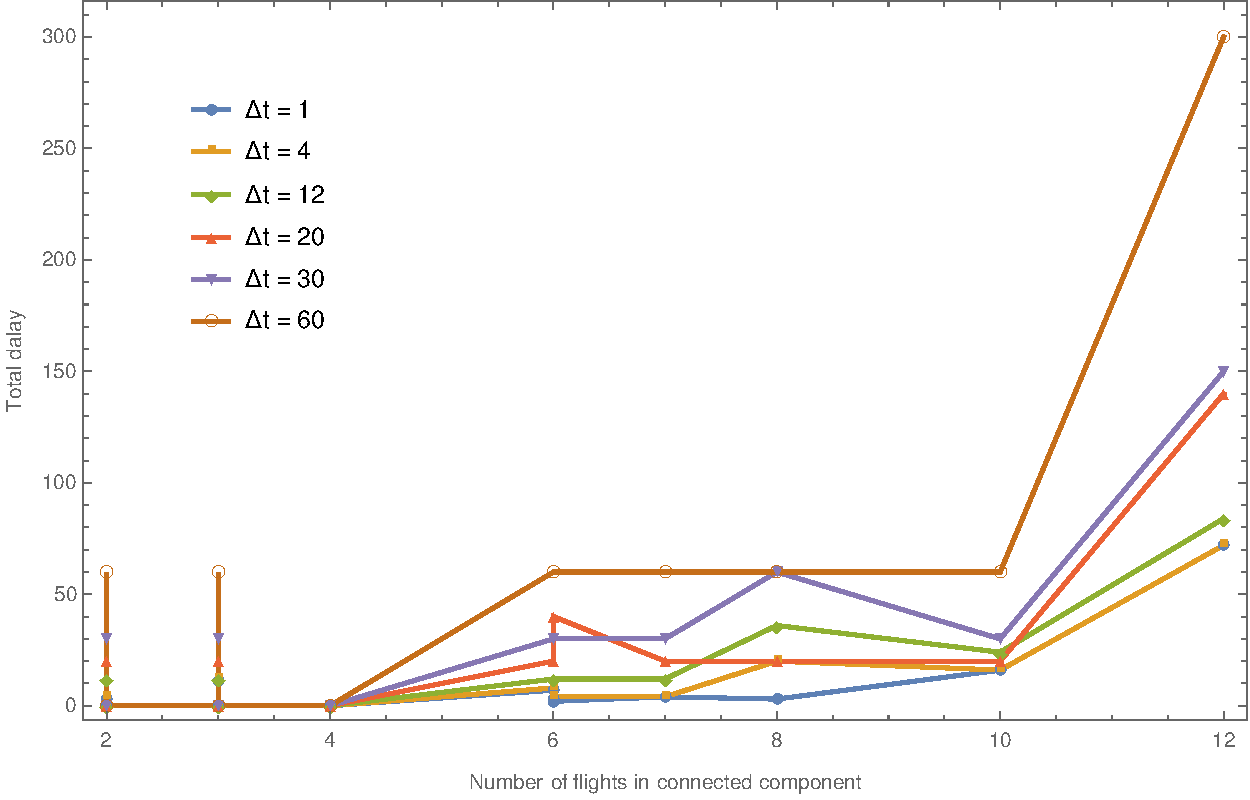
\includegraphics[width=\columnwidth]{pics/qubo_icm/qubo_icm_2.pdf}
  \caption{\label{fig:icm2}. Optimal total delay found by using the Isoenergetic
  Cluster Method (ICM) at fixed time step $\Delta t$ as a function of numbers of
  flight within each connected component. ICM was unable to find solutions for connected
  component with more than $12$ flights.}
\end{figure}

\section{D-Wave}

\subsection{Embedding}

\begin{figure}[htpb]
    \centering
    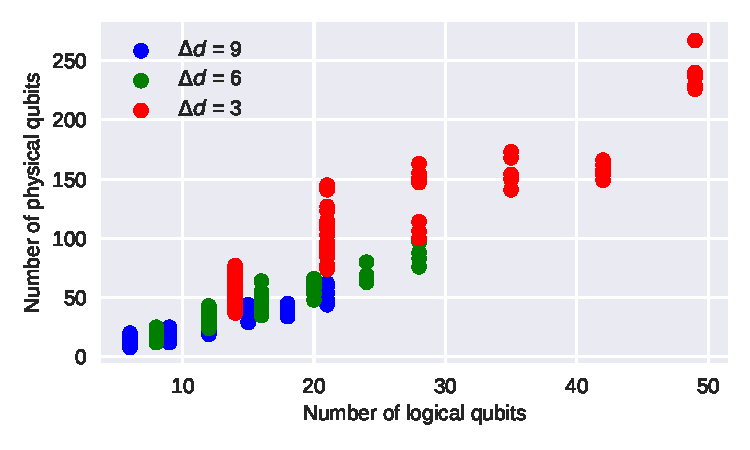
\includegraphics[width=0.45\textwidth]{./pics/physicalVsLogicalNumberOfQubits.pdf}
    \caption{Number of physical qubits versus the number of logical qubits after embedding of QUBO instances with up to $N_f=50$ and $N_c=104$}
\label{fig:number_of_physical_qubits}
\end{figure}

\subsection{Quantum Annealing Results}

\begin{figure}[htpb]
    \centering
    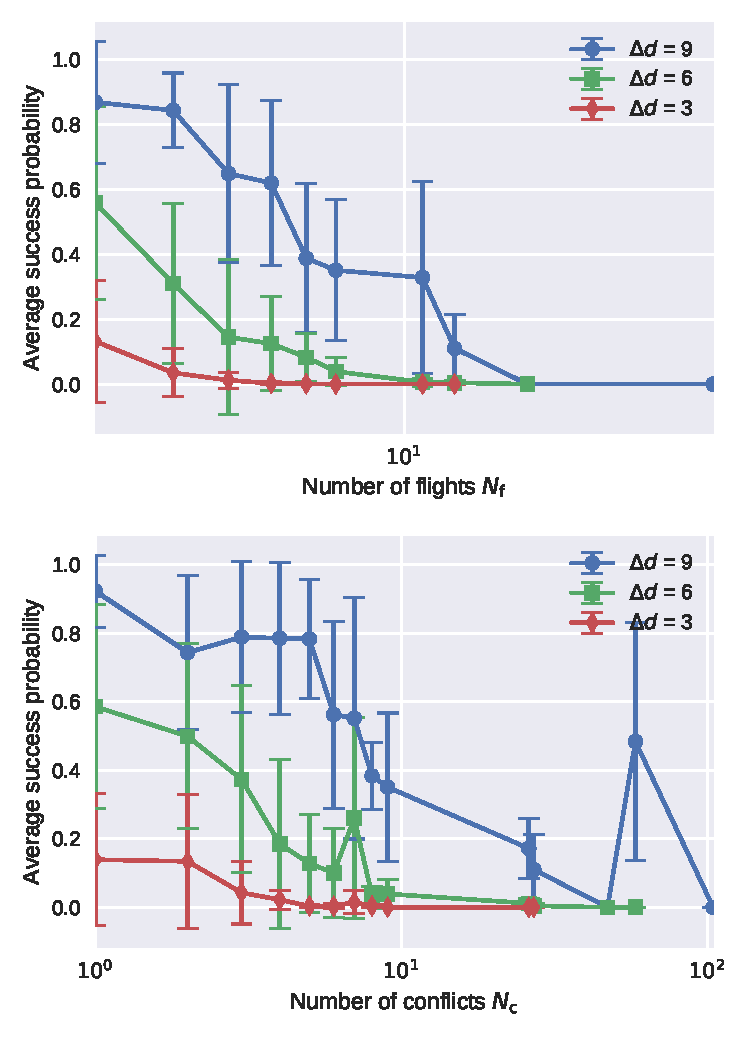
\includegraphics[width=0.45\textwidth]{./pics/annealing_results_success_vs_flights_and_conflicts.pdf}
    \caption{Success probability for QUBO instances in dependence of the number of flights $N_f$ and the number of conflicts $N_c$. 
             The error bars indicate the standard deviation.
             We used $10000$ annealing runs for each instance and penalty weights $\lambda = \lambda_\text{conflict} = \lambda_\text{unique} \in \{0.5, 1, 2\}$. 
    }
\label{fig:success_probability}
\end{figure}

\section{Conclusions}
In this paper, we propose a novel qubo mapping for a simplified version of one
the NASA critical missions: the Air Traffic Management (ATM), i.e. the problem
to find minimal modifications of wind-optimal trajectories to avoid conflicts
between flights. In our study, we considered the actual wind-optimal
trajectories for transatlantic flights (NAT) on July 29, 2012. Given the large
number of flights, it is not a viable solution to directly map the optimal-wind
trajectories in a qubo model. To avoid this bottleneck, our modified version of
the ATM problem is based on the main assumption that flight maneuvers to avoid
conflicts only locally modify the optimal-wind trajectories, with the net effect
to introduce ``delays'' to the flights. Therefore, optimal-wind trajectories can
be ``hard encoded'' in our qubo formulation of the ATM model, leaving the
flights delays as the only variables to optimize. Nevertheless, as explained in
Appendix 2, our method is enough general to potentially include the effect of
maneuvers as well. 

As part of our study, we also introduce a novel ``pre-processing'' algorithm to
eliminate non-potential conflicts that, given a maximum delay, can never occur.
This novel approach is not only important to greatly reduce the number of
potential conflicts (as shown in Section XX), but it also gives an important
indication of the underlying topology the conflict graph. Indeed, we have
discovered that most of the flights have very few conflicts while there are
few flights that have conflicts in a non trivial way. The latter set of flights
represent the hardest part of the ATM problem to optimize. We want to stress
that the proposed pre-processing algorithm is general and can be succesfully
applied for the original ATM problem as well, aiding the already existing
software to improve both the speed and quality to find optimal modification of
the wind-optimal trajectories. 

Finally, we have analyzed the performance of both classical and quantum
heuristics in solving the our qubo model where only delays at the departure are
allowed. Results show that xxx [what can we say here guys?]

In conclusion, we present one of the first attempt to model the Air Traffic
Management problem onto a qubo problem. 

\section{Acknowledgements}


\appendix
\subsubsection{Maneuvers}
A more realistic model of the problem can be created by including maneuvers.
As mentioned above the maneuvers enter our formulation as additional delays $d_{ik}$ at the conflict time.
In the course of mapping to a QUBO formulation, we need to make sure to retain the combinatorial nature of the problem.
We do this by restricting the vast realm of maneuvers to two distinct choices:
Only one of the two involved flights is delayed while leaving the other flight untouched
\begin{equation} \label{eqn:maneuver_model_maneuver_decision}
    \text{if } d_{ik} \neq 0 \Rightarrow d_{jk} = 0  \qquad \forall (i, j) \in I_k \; \forall k \; .
\end{equation}
Moreover, we set the resulting maneuver delays to a constant value $d_M$ large enough to capture all kinds of real maneuvers.
A natural choice for this is the temporal conflict threshold $d_M = \Delta_t$.

With~\eqref{eqn:time_dependent_delay} we can introduce the delay a flight $i$ at the conflict $k$ as
\begin{equation} \label{eqn:maneuver_model_delay_at_conflict}
    D_{ik} = d_i + \sum_{k'<k} d_{ik} \; ,
\end{equation}
where we have defined a temporal ordering of the conflicts for each flight $i$ by
\begin{align*}
                 &k < p \text{ if } t < t' \\
    \text{ for } &t = \min_s x_{i, s} \in C_k \; , \\
                 &t' = \min_s x_{i, s} \in C_p
\end{align*}

The departure delay variables are represented by binary variables as it was done in Section~\ref{sec:departure_delay_model}.
The maneuver delays are given by
\begin{equation*}
    d_{ik} = d_M a_{ik} \qquad a_{ik} \in \{0, 1\}
\end{equation*}
Since the total delay is given by $\sum_{ik} D_{ik}$, we can write the corresponding QUBO contribution as
\begin{equation*}
    \tilde Q_\text{delay} = \sum_{i\alpha} \alpha d_{i\alpha}  + \sum_{ik} d_M a_{ik}\; ,
\end{equation*}

For the conflict avoidance, we need to introduce another variable representing the delay at a given conflict
\begin{equation*}
    D_{ik} = \sum_\delta \delta \Delta_{ik\delta} \qquad \Delta_{ik\delta} \in \{0, 1\} \; .
\end{equation*}
By restricting ourselves to $\Delta_d = \Delta_t$ the values of $\delta$ in the above equation are given as
\begin{equation*}
    \delta \in \{0, \Delta_t, 2\Delta_t, \dots,  (N_d + M_{ik}) \Delta_t\} \; .
\end{equation*}
Here, $M_{ik}$ is the number of conflicts the flight $i$ is involved in before $k$.
In order to fulfill~\eqref{eqn:maneuver_model_delay_at_conflict} we add the following contribution to the QUBO
\begin{equation*}
  \tilde Q_\Delta = \lambda_\Delta \sum_{ik}  {\left( \sum_{\alpha} \alpha d_{i\alpha}  + \sum_{k'<k} d_M a_{ik'} - \sum_\delta \delta \Delta_{ik\delta}\right)}^2 \biggl. \biggr|_{i, j \in I_k}
\end{equation*}
For unique representation of the variables we add 
\begin{align*}
  \tilde Q_\text{unique} = \lambda_\text{unique} & \left\{  \sum_i {\left( \sum_\alpha d_{i\alpha} - 1 \right)}^2 \right. \\
  & \left. + \sum_{ik} {\left( \sum_\delta \Delta_{ik\delta} - 1 \right)}^2 \right\} \; .
\end{align*}
Conflicts are avoided if $D_{ik} - D_{jk} \notin D_k$, $(i, j) \in I_k$. 
The corresponding QUBO contribution reads
\begin{equation*}
    \tilde Q_\text{conflict} = \lambda_\text{conflict} \sum_k \sum_{(\delta, \delta') \in B_k} \Delta_{ik\delta} \Delta_{jk\delta'} \biggl. \biggr|_{i, j \in I_k}
\end{equation*}
where $B_k$ is the set of all $(\delta, \delta')$ which correspond to a conflict
\begin{equation*}
    B_k = \{(\delta, \delta') \; | \; \delta - \delta' \in D_k\}
\end{equation*}
The penalty weights $\lambda_\Delta$, $\lambda_\text{unique}$ and $\lambda_\text{conflict}$ must be chosen large enough to ensure vanishing contributions from the corresponding QUBO terms for the solution.

Finally, the maneuver decision described by~\eqref{eqn:maneuver_model_maneuver_decision} is incorporated by a antiferromagnetic coupling between the two maneuver delay variables
\begin{equation*}
  \tilde Q_\text{maneuver} = J \sum_k  {\left( s_{ik} s_{jk} + 1\right)}_{i, j \in I_k} \; .
\end{equation*}
with 
\begin{equation*}
    s_{ik} = 2 a_{ik} - 1 \in \{-1, 1\}
\end{equation*}
and $J>0$ has to be chosen large enough. 
A solution is considered to be valid only if $\tilde Q_\text{maneuver} = 0$.
Hence, the total QUBO for the maneuver model reads
\begin{equation*}
    Q_\text{MM} = \tilde Q_\text{delay} + \tilde Q_\Delta  + \tilde Q_\text{unique} + \tilde Q_\text{conflict} + \tilde Q_\text{maneuver} 
\end{equation*}

\bibliography{atm}

\end{document}
